\documentclass[psamsfonts]{amsart}

\setlength{\textwidth}{\paperwidth}
\addtolength{\textwidth}{-2in}
\calclayout

\usepackage{comment}
\usepackage{mathrsfs}
\usepackage{amsfonts}
\usepackage{amsmath}
\usepackage{amsthm}
\usepackage{graphicx}
\usepackage{mathrsfs}
\usepackage[dvipsnames]{xcolor}
\usepackage{tikz}
\usepackage{tikz-cd}
\usepackage{amscd}
\usepackage{cancel}
\usepackage{amssymb}
\usepackage{rotating}
\usepackage[colorlinks,citecolor = blue, linkcolor=blue]{hyperref}
\usepackage{bm}
\usepackage[shortlabels]{enumitem}
\usepackage{subcaption}
\usepackage{tablefootnote}

%--------Theorem Environments--------
\theoremstyle{plain}
\newtheorem{thm}{Theorem}[section]
\newtheorem{cor}[thm]{Corollary}
\newtheorem{prop}[thm]{Proposition}
\newtheorem{claim}[thm]{Lemma}


\theoremstyle{definition}
\newtheorem{defn}[thm]{Definition}
\newtheorem{exmp}[thm]{Example}


\theoremstyle{remark}
\newtheorem{rem}[thm]{Remark}
\newtheorem{quest}[thm]{Question}
\newtheorem{remark}[thm]{Remark}

\title{Claims Denials In US Health Insurance}

\author{Mike Gartner}


\begin{document}
	
\maketitle


\begin{abstract}
Claims denials in U.S. health insurance pose a serious problem for consumers
navigating their care. In this report we present and analyze data that sheds
light on the occurrence and prevalence of claims denials, and propose both policies
to improve patient outcomes, and existing avenues for consumer recourse.
\end{abstract}



{
	\hypersetup{linkcolor=black}
	\tableofcontents
}
	

\section{Introduction}
\label{Introduction}
Claims are a fundamental and atomic unit of US health insurance: every time an insured consumer attempts to use their health insurance to cover a portion of a bill, a claim is submitted to their insurer on their behalf. The claim records details about the care received, and the cost of the care. The primary role of health insurers is to receive and adjudicate these claims based on the contracts they sell, and ultimately pay for some portion of them, on behalf of those who purchased the contracts (typically employers or individuals).\\

When insurers adjudicate a claim to determine whether they will pay for it, they review the contracts that govern the coverage which has been purchased on behalf of the insured. The content of these contracts is itself often restricted by various laws and regulations, and the contracts may also include references to external documents (e.g. ``clinical policy bulletins", or ``scientific literature") that are explicitly cited as things that will be used to make coverage determinations. We will say a coverage decision or denial is contractually inappropriate if the decision is inconsistent with the insurance contract governing a policy, or the laws and regulations that apply to that policy.\\

We note that there are many coverage decisions that one might deem morally or medically inappropriate that would not be considered contractually inappropriate. For example, it would be morally reprehensible for corporations with enormous profits to sell policies that completely exclude the use of certain scientifically proven but expensive treatments for those facing dire medical situations, and then to enforce those exclusions despite pleas from patients on their deathbeds. However, such behavior is, unfortunately, not necessarily contractually inappropriate or illegal, depending on the contract in question.\\

The prevalence of contractually inappropriate claims denials, and lack of recourse for consumers even in these cases, have been serious problems for a long time. There are organizations that regularly publish reports \cite{pollitz2021} about the limited publicly available claims denial data that point to this prevalence (e.g. when comparing appeal rates to appeal success rates), and the subject has been discussed in policy research, legal research \cite{fox2010}, and popular journalism \cite{konrad2010} for a long time. Very recently, there have been numerous investigations and articles that have brought to light for the general public just how heinous some of the inappropriate practices taking place really are \cite{armstrong2023a}, \cite{armstrong2023b}. Finally, there are those most seriously affected; many of those with dire, serious, or chronic medical needs (and their friends and families) have long known about the lack of recourse they enjoy, and the frequency with which contractually inappropriate denials occur just in seeking their own care -- they have been on the front lines for decades, suffering the consequences of unregulated corporate greed.\\
	
\subsection{A Primer on Claims Denials}
\hfill\\

\indent A \emph{claim denial} occurs when a claim is submitted to an insurer, and the insurer decides they will not pay for it. In practice, such decisions are made for many reasons; some valid \footnote{\emph{Valid} here could mean medically, morally or contractually valid. We again note that these notions of validity are rarely the same. We will always explicitly qualify the words appropriate or valid if we are specifically referring to a particular notion}, and others inappropriate or indefensible.\\

When a claim is denied, a patient is typically left with an out of pocket expense larger than what they would otherwise face.

\subsection{Measuring Claims Denial Rates}

ne of the most basic metrics that one can use to investigate how claims handling varies is an overall \emph{claims denial rate}. This measures the fraction all claims submitted that are denied:

\begin{equation*}
	\text{Denial Rate} = \dfrac{\text{Claims Denied}}{\text{Claims Received}}
\end{equation*}
\hfill\\
In fact, this is not a uniquely defined notion, because the numerator and denominator can be defined in various ways. For example, one could compute this ratio for all claims submitted to a particular insurer over the course of a year, or for all of the claims submitted for a particular plan over a month, or even for all claims submitted from just one individual to a given plan over the course of a year \footnote{Trying to estimate this last number when choosing an insurer is particularly important for individuals with serious health needs who would be unable to afford the care they need if it were to get denied by their insurer.}. We will calculate denial rates that fit this form from a few different lenses in what follows.\\

It is worth noting that:

\begin{enumerate}
\item A low denial rate is always a good thing for patients, \emph{among the claims that are appropriate} \footnote{Of course not all claims are actually appropriate. For example, sometimes two duplicate claims are submitted for the same care (administratively inappropriate), and approving such claims would in no way help patients. }.
\item High denial rates can be caused by numerous things, and do not always indicate contractually inappropriate insurer practices.
\end{enumerate}


\subsection{Appeals}

When insurers deny claims, patients are often entitled to an appeals process (e.g. those with federal marketplace plans \href{https://www.healthcare.gov/appeal-insurance-company-decision/appeals/}{are afforded such recourse}, as are all others with so-called \emph{non-grandfathered} qualified health plans; see \cite{pollitz2021} for more background).\\

The details of these processes vary based on details of ones insurance plan, but typically they allow patients to initially file an internal appeal of the denial, which is adjudicated by the insurer themselves. If the internal appeal process (which in some plans requires two attempts at an internal appeal) results in the insurer upholding their denial, patients are then often able to file an external appeal. This means they can submit an appeal of the decision to a (purportedly unbiased \footnote{While we do not have evidence to suggest these organizations make determinations in ways biased towards favorable insurer outcomes, we maintain a healthy dose of skepticism about the independence of their decisions, given the landscape of perverse incentives plaguing the entire space. For example, it is unclear to what extent employees migrate between insurance companies and external review agencies. We invite regulators and lawmakers to publish more data publicly supporting the independence and unbiased nature of such agencies. Lack of public consumer access to detailed denial data, including e.g. determination patterns and methodologies among different review agencies, inspires distrust in a system alread plagued by injustices.}) third party, who is responsible for weighing on the decision; insurers are then legally obligated to uphold the final determinations of these third parties. The third parties, and processes by which external appeals are submitted to them and reviewed by them, vary by plan and by state.\\

In understanding the landscape of claims denials, it is useful to understand the frequency of occurrence, and distribution of outcomes, of these appeal processes.\\

\subsubsection{Initial Appeal Rates}

We define the \emph{initial appeal rate} to be the fraction of denied claims that are appealed at the lowest level available to consumers.\\

\begin{equation*}
	\text{Initial Appeal Rate} = \dfrac{\text{Claims Appealed (@ first level)}}{\text{Claims Denied}}
\end{equation*}
\hfill\\

Again, this is a loose definition that we will specify more precisely in each particular calculation below.\\

Of those denials that are internally appealed, we denote the fraction that are overturned by the insurer as the \emph{initial appeal success rate}.\\
	
\begin{equation*}
	\text{Initial Appeal Success Rate} = \dfrac{\text{Claims Overturned (@ first level)}}{\text{Claims Appealed (@ first level)}}
\end{equation*}
\hfill\\
	

\subsubsection{External Appeal Rates}

We define the \emph{external appeal rate} to be the fraction of internally appealed and subsequently upheld denials which are then additionally externally appealed by consumers.\\

\begin{equation*}
	\text{External Appeal Rate} = \dfrac{\text{Claims Appealed Externally}}{\text{Claims Internally Appealed and Upheld}}
\end{equation*}
\hfill\\


Of those denials that are externally appealed, we denote the fraction that are overturned by a third party as the \emph{external appeal success rate}.

\begin{equation*}
	\text{External Appeal Success Rate} = \dfrac{\text{Claims Overturned Externally}}{\text{Claims Appealed Externally}}
\end{equation*}
\hfill\\


\subsubsection{Expected Appeal Phenomenology}

We expect initial appeal success rates to be lower than external appeal success rates, assuming the same population of claims were reviewed \footnote{Note that in practice, one can't compare external and internal appeal success rates directly for the same pool of claims denials. Those appeals that make it to an external review have typically already been through an internal review that was upheld, so the distribution of externally reviewed claims almost never includes e.g. denial cases that an insurer agrees are contractually inappropriate. Presumably, all such cases where an insurer agrees to overturn their initial decision would also be overturned by third parties, if the third parties ever saw them.}. We hold this expectation for two reasons. One is that insurers have a monetary incentive to uphold denials, while third parties do not. The other is that insurers make the initial determinations about what claims to deny, so they obviously have some alignment with the initial denial rationale to begin with. On the other hand, external reviewers may view claims from completely different lenses than that with which an insurer initially viewed them, leading to a higher likelihood of a different conclusion about contractual validity.\\

Finally, we note that both the internal and external appeal systems have the potential to be completely biased, so we should take care to note when we are drawing conclusions from the data that assumes some impartiality in either process. We expect that of all of the data publicly available, external appeal success rates can best inform the underlying validity of (some subset of) initial denials, since at least one third party with no monetary stake in the judgment has been involved in adjudication. Internal appeal data reflects a situation that is opaque by design -- it is difficult to take seriously the purported impartiality of a reviewer that is both reviewing their own decision, and that stands to generate more profit by upholding that decision. There is a reason we don't have juries consisting of the best friends of a defendant.

\subsection{A Dive Into Public Claims Denial Data}

To understand the landscape of claims denials, contractually inappropriate claims denials, appeals, and effective consumer recourse, we need data. Unfortunately for consumers, requirements for insurers to publicly disclose claims denial data are few and far between, and the extent to which requirements that do exist are enforced and regulated is unclear. It would be invaluable for regulators to require broad, transparent claims denial information, and to strictly enforce and audit validity of the data.\\

We make use of a few data sources that are public:\\

\begin{enumerate}
	\item Centers for Medicare and Medicaid Services (CMS) \href{https://www.cms.gov/cciio/resources/data-resources/marketplace-puf}{Public Use Files} (PUFs)\\
	
	Each year CMS releases a collection of transparency data related to federal marketplace insurers. Here we are interested in the \emph{transparency in coverage} \footnote{The term transparency in coverage has been overloaded, and used in different contexts by CMS and other government agencies. Our use of the term here does not refer to the \href{https://www.federalregister.gov/documents/2019/11/27/2019-25011/transparency-in-coverage}{CMS rule published in 2019} requiring health plans to publish certain rate data, which is \href{https://www.cms.gov/healthplan-price-transparency}{broadly being referenced} as the transparency in coverage rule. Instead, it refers only to the \href{https://www.cms.gov/cciio/resources/data-resources/marketplace-puf}{public use files distributed by CMS} documenting federal marketplace denials and appeals (among other things). Note that these are also referred to by CMS as transparency in coverage files, and in fact have been in existence, and referred to in this way, far longer than the TiC rule. Obviously the two efforts are not completely unrelated, and it would be most welcome if reporting requirements in the TiC rule were expanded to incorporate reporting about denial transparency, as do these federal marketplace PUFs. See further discussion in the policy section.} (TIC) public use files. These are files compiled from self-reported insurer data specifying aggregate counts of claims submitted, claims denied, and claims appealed, among other things. This data is limited in scope, and clearly accuracy is not strictly validated based on the frequency of impossible records in the data, but it is the closest thing we have to a denial transparency requirement with broad impact. It is compiled and reported to the public in accordance with the Department of Health and Human Services (HHS) \href{https://www.ecfr.gov/current/title-45/subtitle-A/subchapter-B/part-155/subpart-K/section-155.1040}{rule 45 of the Code of Federal Regulations (CFR), part 155, subpart K} (cf \href{https://www.ecfr.gov/current/title-45/subtitle-A/subchapter-B/part-156/subpart-C/section-156.220}{CFR 156 subpart C)}.\\
	
	
	\item \href{https://www.dfs.ny.gov/reports_and_publications/health_care_claim_reports}{New York Health Care Claim Reports}\\
	
	Thanks to \href{https://www.nysenate.gov/legislation/laws/ISC/345}{legislation from 2020}, New York publishes \href{https://www.dfs.ny.gov/reports_and_publications/health_care_claim_reports}{health care claim reports} for insurance companies (as of plan year 2022) that contain aggregate counts of claims submitted, claims denied, and claims appealed for each NY insurer, among other things. Unfortunately, the data for insurers is not aggregated into a single file, or served in a particularly friendly format for analysis, but we perform this aggregation here and make the transformed data publicly available.\\
	
	
	\item \href{https://www.dfs.ny.gov/public-appeal/search}{New York External Appeal Outcome Data}\\
	
	External appeals of denials from New York marketplace plans, fully insured group plans, and Medicaid managed care plans are adjudicated by Independent Review Organizations. The New York Department of Financial Services manages such appeal processes, and maintains a public database of results from external appeals.\\
	
	
	\item \href{https://fortress.wa.gov/oic/consumertoolkit/Search.aspx?searchtype=indrev}{Washington External Appeal Outcome Data}\\
	
	External appeals of denials from Washington marketplace plans are adjudicated by Independent Review Organizations. According to \href{https://apps.leg.wa.gov/wac/default.aspx?cite=284-43-3030}{Washington Administrative Code 284-43-3030} and the \href{https://app.leg.wa.gov/RCW/default.aspx?cite=48.43.530}{Revised Code of Washington 48.43.530}, insurers must support both internal appeal and external processes, and report resulting data to the insurance commissioner. The code above provides for external appeals to be sought as soon as an internal process is exhausted, or 30 days after internal appeal initiation has occurred, whichever is sooner. Details of the rules pertaining to external appeals are described in the \href{https://app.leg.wa.gov/rcw/default.aspx?cite=48.43.535}{Revised Code of Washington 48.43.535}.\\
	
	The Office of the Insurance Commissioner in Washington state maintains a public database of results from these external appeals.\\
	
	
	\item California External Appeal Data from the \href{https://interactive.web.insurance.ca.gov/apex_extprd/f?p=192:1:2660782937251:::::}{California Department of Insurance (CDI)} and the \href{https://dmhc.ca.gov/AbouttheDMHC/DMHCReports/AnnualReports.aspx}{Department of Managed Health Care (DMHC)}\\
	
	California releases data related to internal and external appeal outcomes in at least four places, all of which we consider:\\
	
	\begin{enumerate}
	\item Yearly CDI \href{https://www.insurance.ca.gov/0400-news/0200-studies-reports/0700-commissioner-report/}{commissioner reports}.\\
	
	These reports include summary statistics, such as the total numbers of claims and internal appeals submitted by consumers. The specific yearly reports we consider here are released by commissioner Ricardo Lara. \\
	
	\item Yearly DMHC \href{https://dmhc.ca.gov/AbouttheDMHC/DMHCReports/AnnualReports.aspx}{secretary reports}.\\
	
	These reports include summary statistics, such as the total numbers of claims and internal appeals submitted by consumers. The specific yearly reports we consider here are released by director Mary Watanabe.\\
	
	\item A \href{https://interactive.web.insurance.ca.gov/apex_extprd/f?p=192:1:5191948876739:::::}{database of Internal Medical Review (IMR) outcomes adjudicated by the California Department of Insurance}.\\
	
	This data corresponds to plans regulated by the CDI.\\
	
	\item A \href{https://data.chhs.ca.gov/dataset/independent-medical-review-imr-determinations-trend}{database of Internal Medical Review (IMR) outcomes pertaining to health maintenance organizations (HMOs)}.\\
	
	This data corresponds to plans regulated by the Caifornia Department of Managed Health Care (DMHC).\\
	
	\end{enumerate}
	
	External appeals (aka internal medical reviews) in California follow processes dictated by two pieces of the California Insurance Code (CIC).\\
	
	\begin{enumerate}
	
	
	\item \href{https://leginfo.legislature.ca.gov/faces/codes_displayText.xhtml?lawCode=INS&division=2.&title=&part=2.&chapter=1.&article=3.5.}{Sections 10169.1 - 10169.5}, which initially became effective January 1, 2001, describe rules that apply to IMR sought for health coverage decisions purportedly related to medical necessity. There have been numerous modifications to the law since then. The current law expressly provides for the inclusion of those on Medicare and Medicare Advantage plans, however it also allows for processes to be subsumed by existing state Medicare resolution outlets. It allows IMRs to be sought as soon as an internal process is exhausted, or 30 days after internal initiation has occurred, whichever is sooner. It also allows the CDI to contract with the DMHC to administer the IMR as desired (which has come into play for managed care plans, such as HMOs, as described in the last dataset description above.)\\
	
	\item \href{https://leginfo.legislature.ca.gov/faces/codes_displaySection.xhtml?lawCode=INS&sectionNum=10145.3.}{Section 10145.3}, also effective as of January 1, 2001, describes particular rules that apply to IMR sought for insurer decisions stemming from deeming treatment or services as experimental or investigational in nature.\\
	
	\end{enumerate}
	
	
	\item Connecticut Denial Data From \href{https://portal.ct.gov/CID/Reports/Consumer-Report-Card-on-Health-Insurance-Carriers-in-Connecticut}{Consumer Report Cards}
	
	Connecticut's state Department of Insurance releases a report, the so called Consumer Report Card on Health Insurance Carriers, each year. The report includes various aggregate statistics about health insurance plans, including utilization for certain services, member satisfaction, and aggregate denial statistics.\\
\end{enumerate}
	
To our knowledge, this is the first report that compiles aggregate results across a wide array of disparate sources containing claims denial data.\\

An overview of the data we analyze in this report is detailed in Table \ref{summarytable} below.

	\begin{table}[!ht]
	\centering
	\begin{tabular}{|p{3cm}|p{4cm}|p{2cm}|p{2cm}|p{4cm}|}
		\hline
		\textbf{Data Source (plan years considered)} & \textbf{Market Segment} & \textbf{Num Denials} & \textbf{Denials Represented} & \textbf{Consumer Population Represented}  \\ \hline
		CMS TIC PUF (2021) & Federal marketplace & 48,302,001 & All & 8,251,703 \\ \hline
		NY Health Care Claims Reports (2022) & All NY Issuers & 25,996,601 & All & Unknown, but $\geq$ 5,000,000 \tablefootnote{It is unclear which exact pool of insurance plans, and therefore consumers, this data covers. It appears the DFS has jurisdiction to regulate external appeals for all individual marketplace plans, fully insured group plans, and Medicaid managed care plans. We planned to estimate this population using the \href{https://www.dfs.ny.gov/system/files/documents/2022/08/ny_consumer_guide_health_insurers_2022.pdf}{DFS consumer report for the 2021 plan year}, but found it does not include enrollment. In fact, we couldn't even corroborate the denial numbers from the 2021 plan year from the aforementioned report, and found a significant discrepancy between the total number of external denials listed in that report, and the number that exist in the DFS database. We belive this discrepancy comes from the fact that the report excludes summary statistics for numerous categories of smaller plans, such as HMOs with less than 500 members, and commercial and EPO/PPO plans with less than 50 million in premiums.
			
			However, we can say that the population of consumers corresponding to plans that the DFS regulates at least includes marketplace plans, and according to New York State of Health \href{https://info.nystateofhealth.ny.gov/enrollmentdata}{enrollment data}, that population has hovered between 4.5-7 million over the years represented here.}  \\ \hline
		NY External Appeals Database (2019-2023) & NY marketplace, fully insured group plans, and Medicaid managed care plans & 26,036 & Externally Appealed (IMR) & Unknown, but $\geq$ 5,000,000  \\ \hline
		WA External Appeals Database (2016-2023) & WA marketplace & 8774 & Externally Appealed (IMR) & 222,731  \\ \hline
		CA DOI External Appeals Database (2011-2023) & CA marketplace, and fully insured group plans & 4,658 & Externally Appealed (IMR) & 852,506 \tablefootnote{We use the total enrollment noted in the \href{https://www.insurance.ca.gov/0400-news/0200-studies-reports/0700-commissioner-report/}{2021 CDI report}, since it is explicitly noted. This number is therefore relevant for the subset of the database containing IMRs from 2021, but not other years, since the consumer population in this market segment changes yearly. }  \\ \hline
		CA DMHC External Appeals Database (2001-2023) & Large group and self funded plans regulated by DMHC & 34,615 & Externally Appealed (IMR) & 23,474,332 \tablefootnote{We use the total enrollment noted in the \href{https://dmhc.ca.gov/AbouttheDMHC/DMHCReports/AnnualReports.aspx}{2021 DMHC secretary report}, since it is explicitly noted. This number is therefore relevant for the subset of the database containing IMRs from 2021, but not other years, since the consumer population in this market segment changes yearly.}  \\ \hline
		Connecticut Consumer Report Card (2021) & All CT issuers (excluding government sponsored) & 2,708,724 & All & 1,991,903 \tablefootnote{We use the total enrollment noted in the \href{https://portal.ct.gov/CID/Reports/Consumer-Report-Card-on-Health-Insurance-Carriers-in-Connecticut}{2021 consumer report card}, since it is explicitly noted.}  \\ \hline
	\end{tabular}
\caption{Summary of Datasets Considered}
\label{summarytable}
\end{table}
	

\subsection{Federal Marketplace Insurers}
\hfill\\
\indent Using CMS TIC PUF data, we analyzed the landscape of federal marketplace denials and appeals from 2021 \footnote{Note that the CMS TIC PUF data is reported and labeled two years later than the date to which it corresponds. Thus the 2021 data is labeled by CMS as the 2023 TIC PUF.}. The data suggests denials are generally prevalent, while appeals of all forms are scarce. For those that do appeal, however, overturn rates are high. \\

\subsubsection{Initial Denial Rates}
\hfill\\

Of note, 16\% of all federal marketplace claims submitted in 2021 were initially denied. The data is displayed in Figure \ref{federal_denial_rate}.\\

\begin{figure}
	\centering
	\textbf{Aggregate Claims Denial Rate, Federal Marketplace Insurers, 2021}\par\medskip
	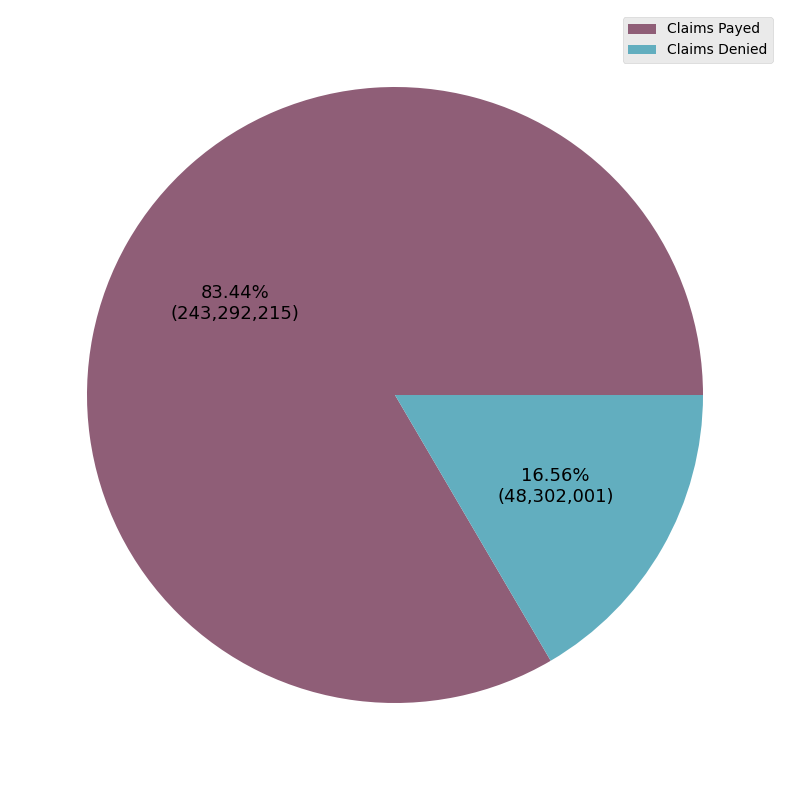
\includegraphics[width=0.85\columnwidth]{images/cms_puf/overall_denial_pie.png}
	\caption{Aggregate denial rate across federal marketplace insurers in 2021. Approximately 16\% of all federal marketplace claims were initially denied in 2021, according to CMS TIC PUF data. Source: CMS TIC PUF data.}
	\label{federal_denial_rate}
\end{figure}


The distribution of denial rates across insurers, plans, plan types, and regions varies drastically. Figure \ref{federal_denial_rate_hist} shows the distribution of overall issuer denial rates across issuers represented in the 2021 CMS TIC PUF data. The distribution is bimodal, with a large majority of issuers comprising a contingency with aggregate denial rates between 0\% to 30\%, and a small contingency of issuers maintaining aggregate denial rates between 35\% to 50\%.

\begin{figure}
	\centering
	\textbf{Claims Denial Rates Across Federal Marketplace Issuers, 2021}\par\medskip
	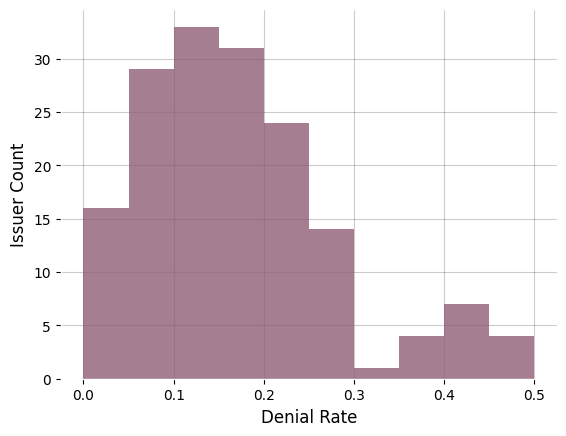
\includegraphics[width=0.85\columnwidth]{images/cms_puf/denial_rates_all_insurers.png}
	\caption{Distribution of claims denial rates across federal marketplace issuers in 2021. Across issuers, denial rates vary from approximately 0\% to 50\%. Source: CMS TIC PUF data.}
	\label{federal_denial_rate_hist}
\end{figure}

Federal marketplace plans included in this CMS TIC PUF data sometimes report rationales for claim denials. When reported, the available options for these rationales are:\\

\begin{enumerate}
	\item Referral Required
	\item Out of Network
	\item Services Excluded
	\item Not Medically Necessary
	\item Other
\end{enumerate}

Most denials logged in the CMS PUF data are associated with a rationale of "Other" (see Figure \ref{federal_denials_by_rationale}), which provides little information to the public.\\

\begin{figure}
	\centering
	\textbf{Claims Denials By Rationale, Federal Marketplace Issuers, 2021}\par\medskip
	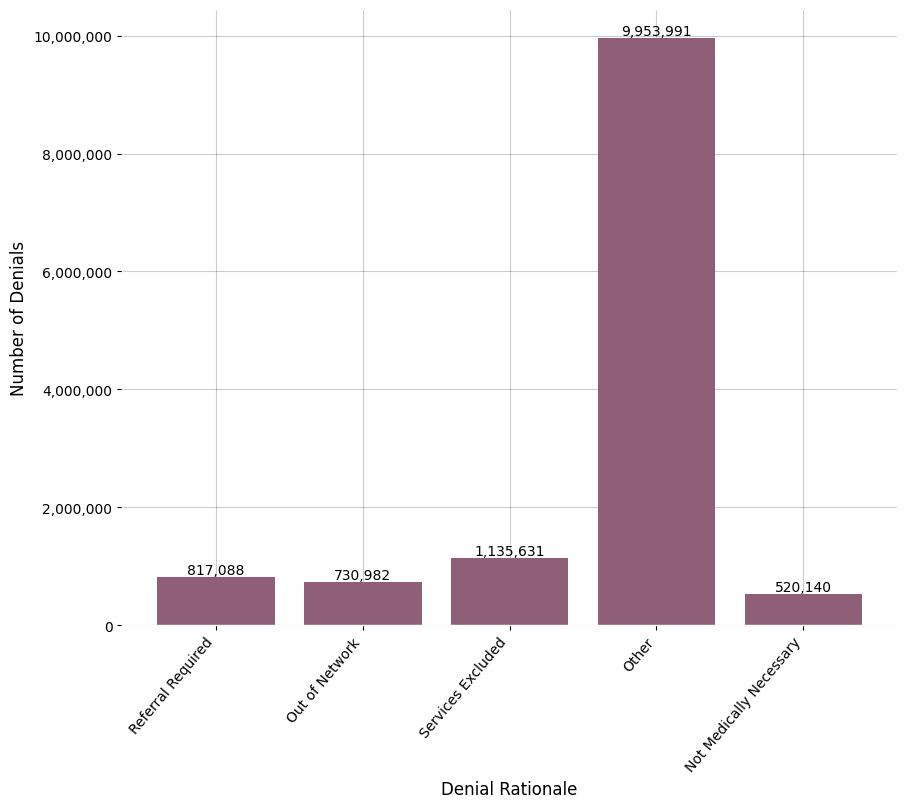
\includegraphics[width=0.85\columnwidth]{images/cms_puf/denials_by_rationale.png}
	\caption{Distribution of claims denial rationales in a subset of the TIC PUF data. Denial rationales are reported at the plan level, and we only included here those plans which reported denial rationales which either summed to the total number of denials reported, or which summed to this value when excluding out of network denials. We could not resolve whether the other data could be trusted by any reporting standard. Source: CMS TIC PUF data.}
	\label{federal_denials_by_rationale}
\end{figure}

Effectively, this reporting scheme allows insurers to withhold reporting the actual reason for a denial to the public if they so choose, since it is not completely clear what is allowed to be reported in this bucket, and there is no strict validation of the reported data. Whether or not insurers actually abuse this system cannot be gleaned from this data alone.\\


Figure \ref{federal_denial_map} shows the average issuer level claims denial rates for each region represented in the CMS TIC PUF data. We also present a more comprehensive summary of the data in Table \ref{federal_denial_data_by_region_table}\\

\begin{figure}
	\centering
	\textbf{Claims Denial Rates By Region, Federal Marketplace Issuers, 2021}\par\medskip
	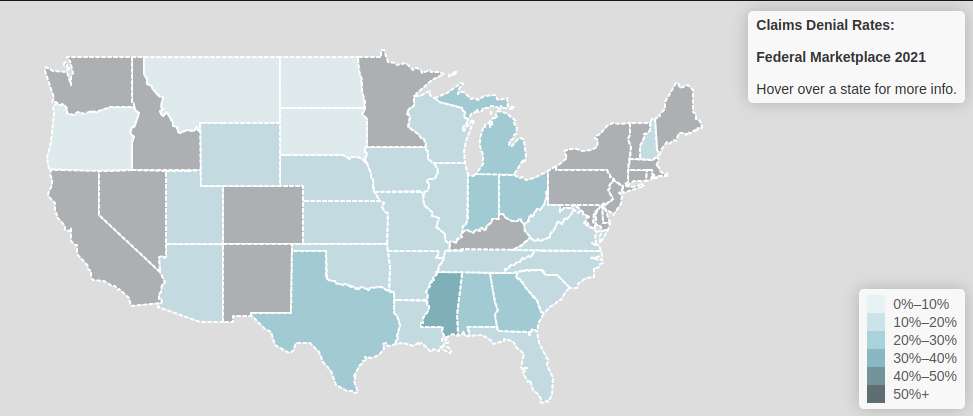
\includegraphics[width=0.85\columnwidth]{images/cms_puf/federal_denial_rates.png}
	\caption{Claims denial rates broken down by region. Source: CMS TIC PUF data.}
	\label{federal_denial_map}
\end{figure}

Among this federal marketplace data, Mississippi stands out for having a uniquely high aggregate denial rate, with Texas, Alabama, Alaska, Georgia, Ohio, Indiana and Michigan occupying the next batch of worst offenders. In many regions, a relatively small collection of issuers contribute a majority of the claims denied.\\


\begin{table}[!ht]
	\centering
	\begin{tabular}{|p{3cm}|p{2cm}|p{2cm}|p{2cm}|p{3cm}|p{2cm}|}
		\hline
		State or Region & Denial Rate & Claims Received & Claims Denied & Number of Consumers & Number of Insurers \\ \hline
		Alaska & 0.235 & 611313 & 143836 & 16707 & 2 \\ \hline
		Alabama & 0.224 & 7657061 & 1716993 & 168717 & 2 \\ \hline
		Arkansas & 0.185 & 15180958 & 2808497 & 59629 & 5 \\ \hline
		Arizona & 0.192 & 3612118 & 694976 & 115409 & 6 \\ \hline
		Florida & 0.131 & 75588407 & 9868686 & 1867568 & 10 \\ \hline
		Georgia & 0.289 & 10825149 & 3127963 & 387441 & 6 \\ \hline
		Hawaii & 0.244 & 486179 & 118578 & 16343 & 2 \\ \hline
		Iowa & 0.149 & 2828360 & 421458 & 40699 & 3 \\ \hline
		Illinois & 0.176 & 10755531 & 1893905 & 248363 & 7 \\ \hline
		Indiana & 0.236 & 4233263 & 997114 & 91625 & 3 \\ \hline
		Kansas & 0.135 & 2333613 & 314062 & 43716 & 5 \\ \hline
		Louisiana & 0.151 & 5040194 & 761581 & 78236 & 4 \\ \hline
		Michigan & 0.205 & 7783687 & 1599048 & 138398 & 8 \\ \hline
		Missouri & 0.191 & 6173944 & 1182181 & 113034 & 8 \\ \hline
		Mississippi & 0.381 & 1411877 & 537222 & 50769 & 2 \\ \hline
		Montana & 0.096 & 1379424 & 132490 & 41233 & 3 \\ \hline
		North Carolina & 0.125 & 26446640 & 3295778 & 284269 & 5 \\ \hline
		North Dakota & 0.042 & 1873450 & 77936 & 21803 & 3 \\ \hline
		Nebraska & 0.102 & 3305776 & 338692 & 48619 & 2 \\ \hline
		New Hampshire & 0.184 & 1436531 & 264608 & 34360 & 3 \\ \hline
		Ohio & 0.217 & 5795555 & 1255800 & 138349 & 10 \\ \hline
		Oklahoma & 0.163 & 8986426 & 1461998 & 138695 & 4 \\ \hline
		Oregon & 0.07 & 1999967 & 139605 & 111343 & 6 \\ \hline
		South Carolina & 0.18 & 10502152 & 1885641 & 179317 & 3 \\ \hline
		South Dakota & 0.057 & 776818 & 44532 & 25419 & 2 \\ \hline
		Tennessee & 0.18 & 11196451 & 2011182 & 140672 & 6 \\ \hline
		Texas & 0.204 & 35256067 & 7201165 & 591074 & 10 \\ \hline
		Utah & 0.138 & 10086291 & 1391050 & 151905 & 6 \\ \hline
		Virginia & 0.164 & 9224112 & 1508696 & 224605 & 9 \\ \hline
		Wisconsin & 0.117 & 5952081 & 694105 & 128863 & 13 \\ \hline
		West Virginia & 0.162 & 883377 & 143100 & 7069 & 2 \\ \hline
		Wyoming & 0.128 & 1157244 & 148487 & 26777 & 2 \\ \hline
	\end{tabular}
\caption{Summary of Federal Marketplace Denial Data, Broken Down By Region}
	\label{federal_denial_data_by_region_table}
\end{table}

\subsubsection{Internal Appeals}

The data are striking in that they make clear that while appeals of all forms are extremely rare among marketplace consumers, those that do appeal have a high appeal success rate. Figure \ref{federal_internal_appeal_rates} shows the fraction of initially denied claims that are appealed by consumers, while Figure \ref{federal_internal_appeal_success_rates} shows the fraction of appeals
that are overturned.\\

\begin{figure}
	\centering
	\textbf{Internal Appeal Rates, Federal Marketplace Issuers, 2021}\par\medskip
	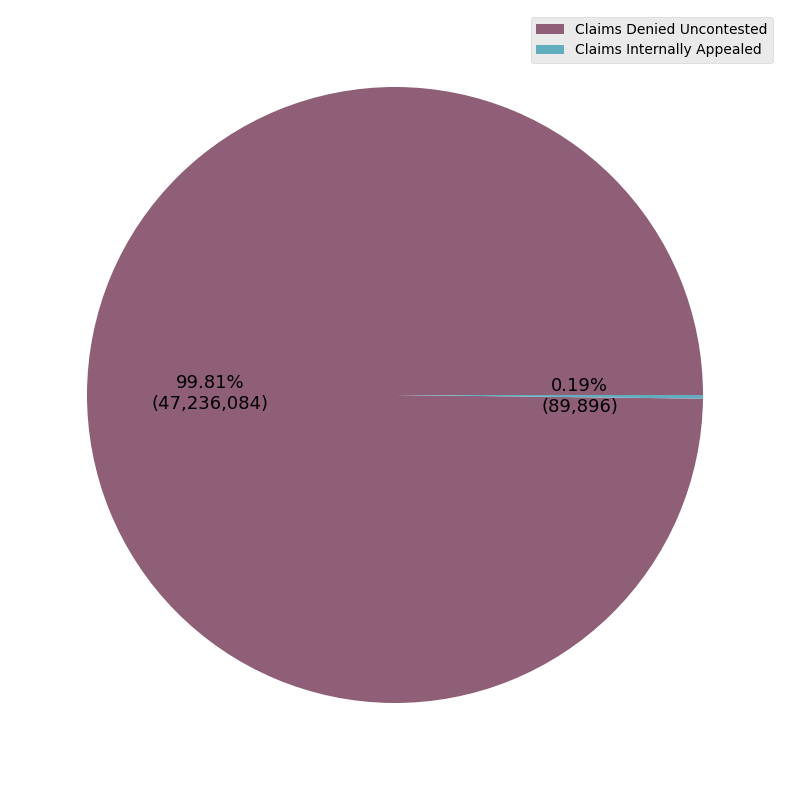
\includegraphics[width=0.85\columnwidth]{images/cms_puf/internal_appeal_rates_all_insurers.png}
	\caption{ Internal appeal rates among federal marketplace issuers in 2021. Only 1/5 of a percent of the approximately 50 million initially denied claims are appealed. Source: CMS TIC PUF data.}
	\label{federal_internal_appeal_rates}
\end{figure}


\begin{figure}
	\centering
	\textbf{Internal Appeal Success Rates, Federal Marketplace Issuers, 2021}\par\medskip
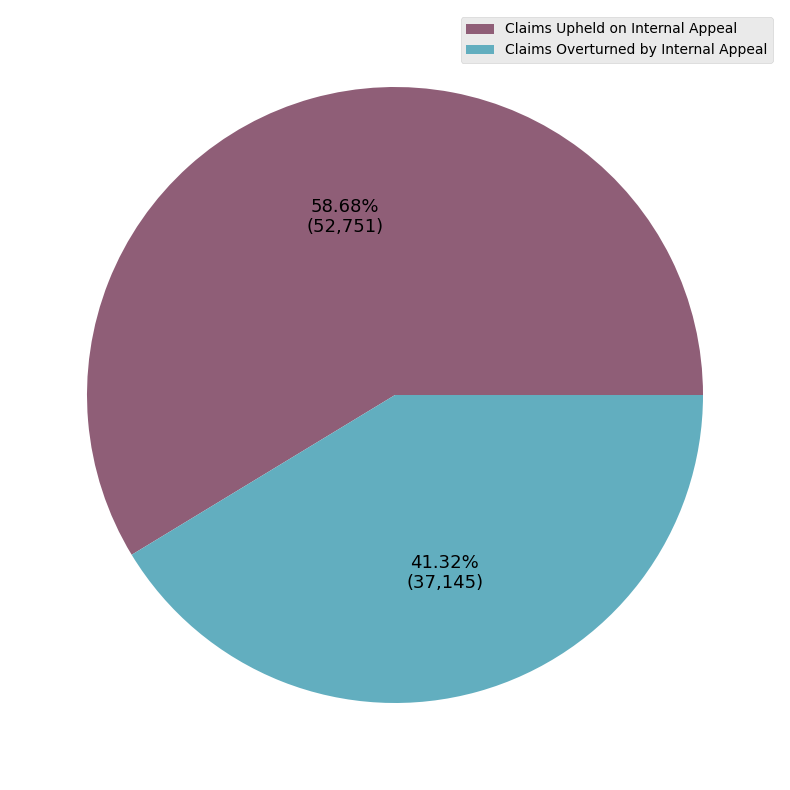
\includegraphics[width=0.85\columnwidth]{images/cms_puf/internal_appeal_success_rates_all_insurers.png}
	\caption{ Internal appeal success rates among federal marketplace issuers in 2021. Only 1/5 of a percent of the approximately 50 million initially denied claims are appealed, but of those that are, 41 percent get immediately overturned on a first level internal review. Source: CMS TIC PUF data.}
	\label{federal_internal_appeal_success_rates}
\end{figure}


The initial appeal rate is about .2\%, while the initial success rate among internally appealed claims is about 41\%. We note that the disparity between the fraction of denials being appealed and the fraction of those appeals being internally overturned could be rooted in various phenomenon \footnote{For example, it could be the case that the distribution of cases being internally appealed are those that are particularly egregious or obvious inappropriate denials, and that the expected appeal success rate would drop drastically if one were to appeal every denial with the adjudication processes remaining fixed.}. Nonetheless, it is informative to consider what this disparity would imply under different assumptions. \\

Let's consider what would happen if more federal marketplace insurer denials were appealed. Suppose:

\begin{enumerate}
\item The fraction of denials appealed initially is X\% (X=.1899506X=.1899506\% in the data above).
\item The initial appeal success rate is Y\% (Y=41.32Y=41.32\% in the data above).
\item The average value per denied claim is \$Z (we do not have enough information to estimate Z for this distribution of claims data).
\end{enumerate}

Note that even for a highly conservative estimate, scaling appeal rates has high value implications. For example, scaling currently observed internal appeal success rates (41.32\%) to 1\% of all denied claims on the federal marketplace with an average value per claim of just \$10 (X=1, Y=41.32, Z=10), would result in approximately 150k extra overturned claims and an extra 1.5 million USD of value returned to consumers.\\

This does not include all of the insurance denials that occur outside of the federal marketplaces, or those that were not reported in this incomplete data, nor does it take into account the fact that external appeals are a less biased process that data suggests would lead to even more overturns.\\

The takeaway is that consumers should be appealing inappropriate denials whenever possible, and we need organizations, regulators, and individuals to support consumers and aid them in scaling the rate at which they are following through with such appeals when faced with contractually inappropriate denials.\\

The monetary value alone is significant to consumers, and there are many important additional implications for their health (see Section \ref{policy_section} below for more details).\\


\subsubsection{External Appeals}

In Figures \ref{federal_external_appeal_rates} and \ref{federal_external_appeal_success_rates} we display the external appeal rates and external appeal success rates from the CMS TIC PUF data.\\



\begin{figure}
	\centering
	\textbf{External Appeal Rates, Federal Marketplace Issuers, 2021}\par\medskip
	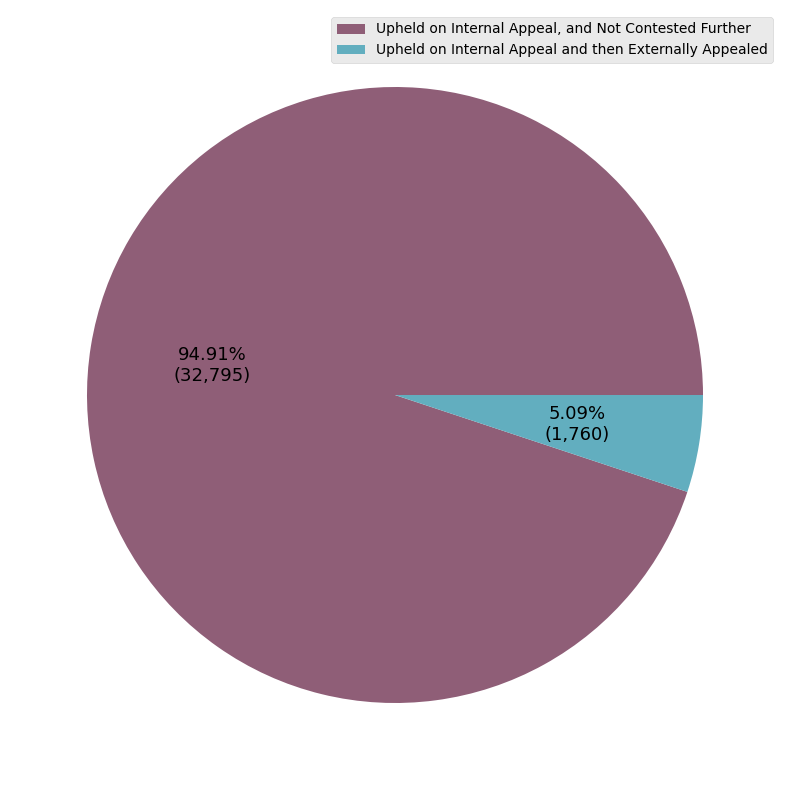
\includegraphics[width=0.85\columnwidth]{images/cms_puf/external_appeal_rates_all_insurers.png}
	\caption{External appeal rates among federal marketplace issuers that reported the data in 2021. Not all issuers and plans reported external appeal data in the CMS PUF. Among the issuers reporting external appeal data, only 5 percent of the approximately 34 thousand denials upheld on internal appeal are externally appealed Source: CMS TIC PUF data.}
	\label{federal_external_appeal_rates}
\end{figure}

\begin{figure}
	\centering
	\textbf{External Appeal Success Rates, Federal Marketplace Issuers, 2021}\par\medskip
	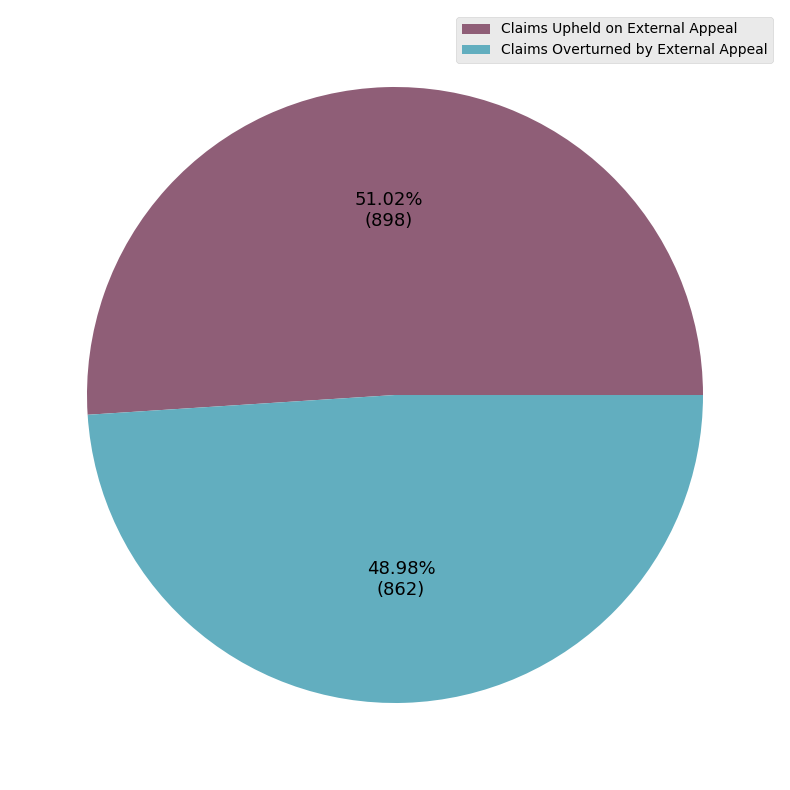
\includegraphics[width=0.85\columnwidth]{images/cms_puf/external_appeal_success_rates.png}
	\caption{External appeal success rates among federal marketplace issuers that reported the data in 2021. Not all issuers and plans reported external appeal data in the CMS PUF. Among the issuers reporting external appeal data, only 5 percent of the approximately 34 thousand denials upheld on internal appeal are externally appealed, but of those, nearly 49 percent get overturned when reviewed by an independent external agency. Source: CMS TIC PUF data.}
	\label{federal_external_appeal_success_rates}
\end{figure}

A key fact to take away from the external appeal data is the rate at which claims that are denied, and then subsequently re-reviewed internally by insurers on request, and finally upheld as denials, are then overturned when reviewed by impartial expert third parties with no monetary stake in the decision outcome. Of the 1760 claims represented in this data that were denied, internally appealed, upheld as denials, and then externally appealed, a staggering 49\% were deemed by external reviewers to be inappropriate.\\

This result clearly shows that internal review processes cannot be trusted to be impartial, fair, or adjudicate appropriately.\\

Internal processes are, effectively, a means by which regulators and insurers force consumers to jump through hoops before receiving unbiased consideration. The insurers understand this data well (and if they claim they do not, they are at best grossly negligent for not understanding this data), and know that most consumers will never jump through the last hoop to access their right to an independent external review (evidently 95\% of the consumers in this data who make it to the second to last hoop don't have the wherewithal to make it to the last hoop).\\


\subsection{New York Health Care Claims Reports}



\subsection{Acknowledgements}
It is a pleasure to thank the following people for their support and guidance in reviewing this manuscript:



\bibliographystyle{alpha}
\bibliography{References}

	
\end{document}
